\clearpage
\section{Living Systematic Reviews with \name{} for 9 Priority Pathogens}\label{app:report_writeup}

Utilising \name{} on the data extracted corpus from previous stages, we generated living reviews for nine WHO priority pathogens: Marburg virus, Ebola virus, Lassa virus, SARS-CoV-1, Zika virus, MERS-CoV, Nipah virus, Rift Valley fever (RVF) virus, and Crimean--Congo haemorrhagic fever (CCHF) virus. Each review comprises two complementary documents (a transmission-modelling review synthesising extracted model characteristics, and an outbreak surveillance review aggregating historical outbreak data) alongside structured datasets and visualisations. While four of these pathogens (Ebola, Lassa, SARS, Zika) have been validated against PERG's expert annotations as described in \cref{sec:human_expert_validation}, the remaining five represent preliminary syntheses for pathogens where PERG's systematic review process has not yet commenced or is in early stages.

Figure~\ref{fig:ebola_reviews} presents excerpts from the Ebola living reviews, illustrating the structure and content of \name{}'s outputs for a validated pathogen. The transmission-modelling review (Figure~\ref{fig:ebola_models}) provides a quantitative overview of the $513$ extracted models, including distributions across model architectures, stochasticity classifications, and code availability. The outbreak surveillance review (Figure~\ref{fig:ebola_outbreaks}) synthesises $1,104$ outbreak records spanning nearly six decades, with temporal coverage, geographic distribution, and detection methodology patterns presented through evidence-based descriptions paired with interpretive commentary blocks.

\begin{figure}[h]
    \centering
    \begin{subfigure}[t]{0.6\textwidth}
        \centering
        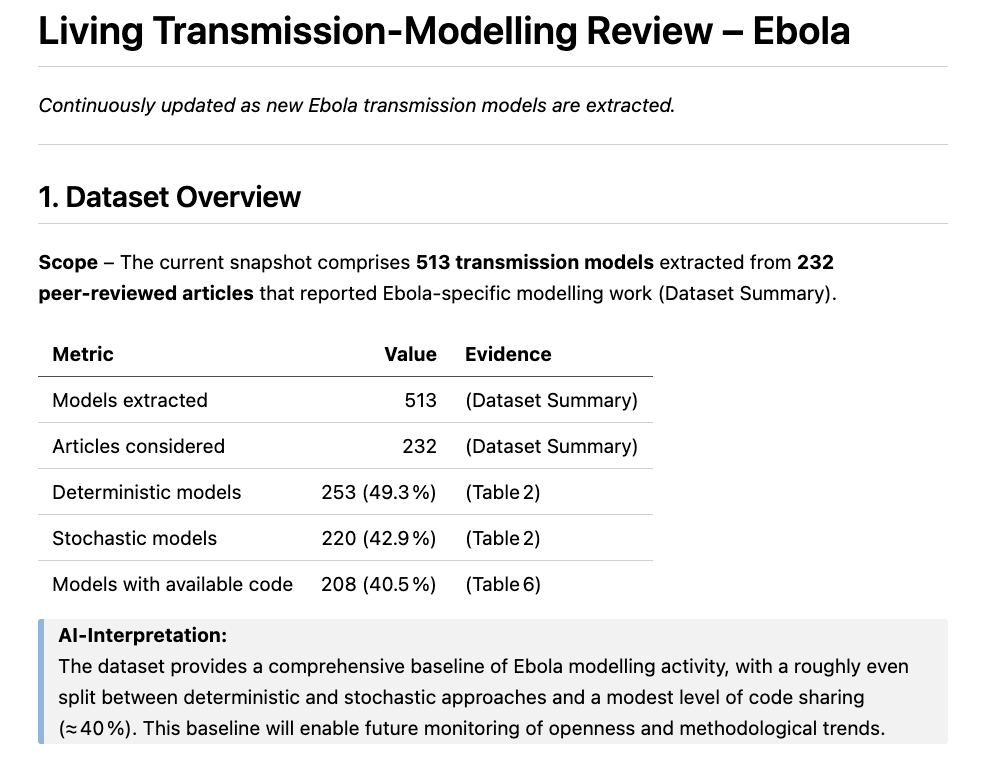
\includegraphics[width=0.6\textwidth]{figures/report_generation/EBOLA_MODELS.png}
        \caption{Transmission-Modelling Review excerpt showing dataset scope, model architecture distribution, and reproducibility indicators for $513$ Ebola models extracted from $232$ articles.}
        \label{fig:ebola_models}
    \end{subfigure}

    \vspace{0.5em} % optional spacing between figures

    \begin{subfigure}[t]{0.6\textwidth}
        \centering
        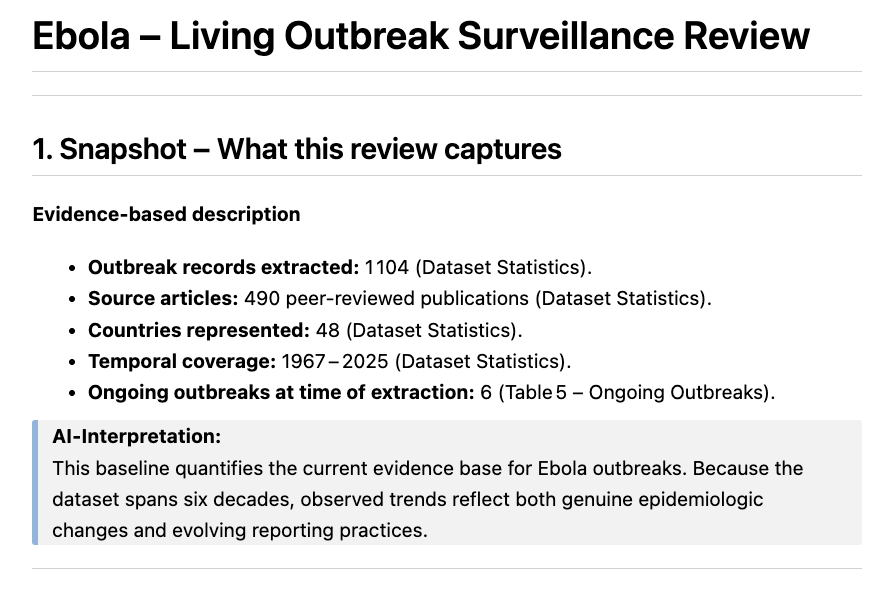
\includegraphics[width=0.6\textwidth]{figures/report_generation/EBOLA_OUTBREAKS.png}
        \caption{Outbreak Surveillance Review excerpt presenting snapshot statistics for $1,104$ outbreak records from $490$ publications, covering temporal span 1967--2025 and $48$ countries.}
        \label{fig:ebola_outbreaks}
    \end{subfigure}

    \caption{\textbf{Ebola living reviews generated by \name{}.} Both reviews follow a structured format: evidence-based descriptions citing supporting figures and tables, followed by interpretation blocks explicitly labelled as AI-generated synthesis. Ebola represents one of four pathogens validated against PERG expert annotations (\cref{sec:human_expert_validation}).}
    \label{fig:ebola_reviews}
\end{figure}
For emerging or understudied pathogens, rapid synthesis of available evidence can inform outbreak preparedness even when comprehensive expert review remains infeasible. Figure~\ref{fig:unvalidated_reviews} presents excerpts from RVF and CCHF reviews, two pathogens for which PERG has not yet initiated systematic screening. The RVF transmission-modelling review (Figure~\ref{fig:rvf_models}) characterises $115$ models extracted from the retrieved literature, revealing a predominance of compartmental architectures and vector-to-human transmission pathways consistent with RVF's arboviral ecology. The CCHF outbreak surveillance review (Figure~\ref{fig:cchf_outbreaks}) maps $59$ outbreak records with quantitative case data, identifying geographic clusters and temporal patterns across affected regions. While these syntheses lack the validation rigour applied to Ebola, Lassa, SARS, and Zika, they demonstrate \name{}'s capacity to generate preliminary evidence summaries for resource allocation and hypothesis generation in under $48$ hours of wall-clock time.

\begin{figure}[h]
    \centering
    \begin{subfigure}[t]{0.48\textwidth}
        \centering
        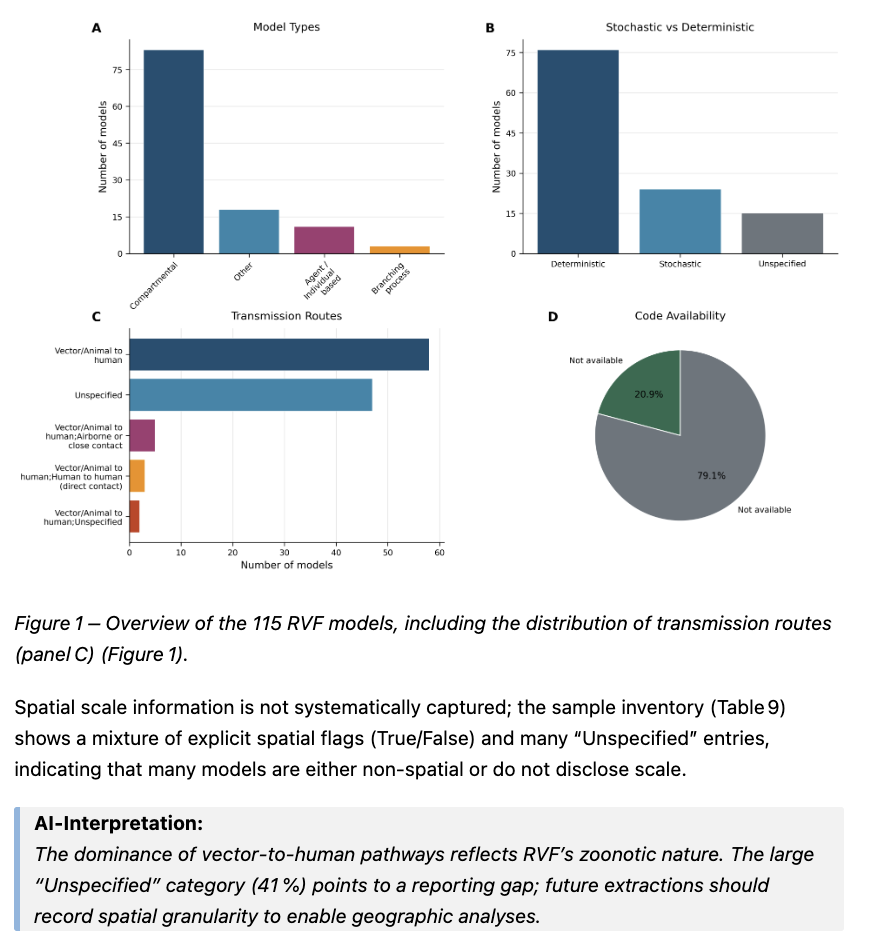
\includegraphics[width=\textwidth]{figures/report_generation/RVF.png}
        \caption{RVF transmission-modelling review showing distribution of $115$ extracted models across architecture types, stochasticity, transmission routes, and code availability.}
        \label{fig:rvf_models}
    \end{subfigure}
    \hfill
    \begin{subfigure}[t]{0.48\textwidth}
        \centering
        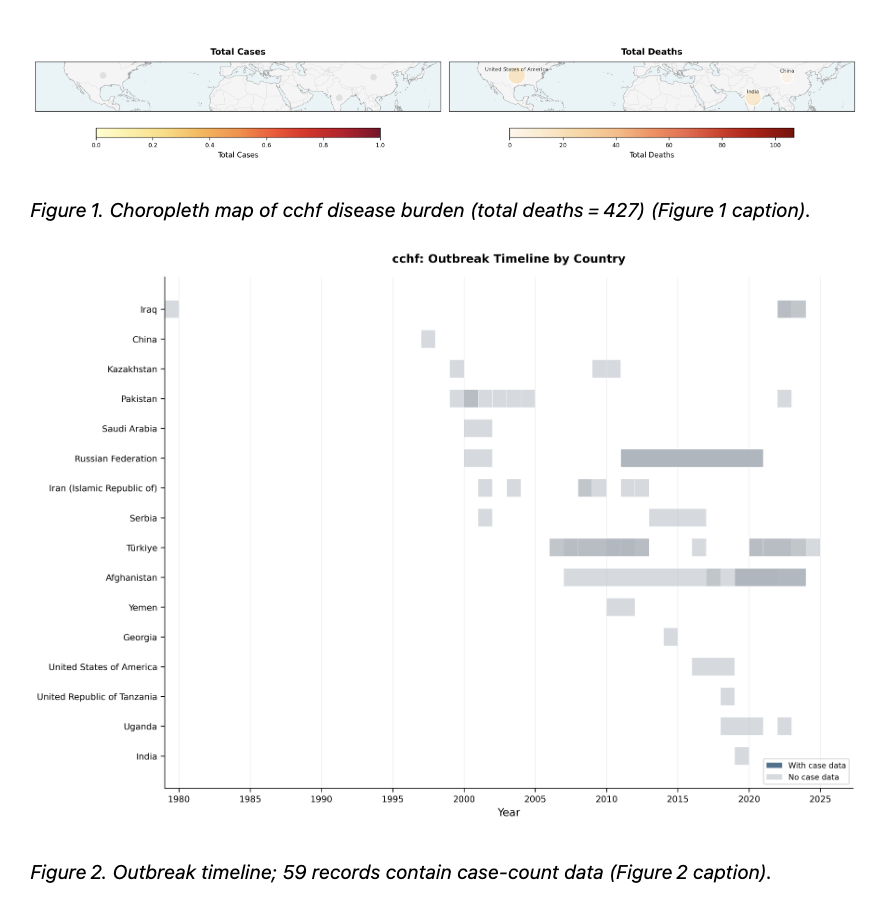
\includegraphics[width=\textwidth]{figures/report_generation/CCHF.png}
        \caption{CCHF outbreak surveillance review presenting geographic burden (choropleth maps) and temporal distribution of $59$ outbreaks with case-count data.}
        \label{fig:cchf_outbreaks}
    \end{subfigure}
    \caption{\textbf{Preliminary living reviews for pathogens without completed PERG validation.} RVF and CCHF represent pathogens for which PERG has not yet commenced systematic screening. These \name{}-generated reviews provide initial evidence synthesis for outbreak preparedness planning, though they lack the expert validation applied to the four evaluated pathogens (Ebola, Lassa, SARS, Zika).}
    \label{fig:unvalidated_reviews}
\end{figure}


Table~\ref{tab:review_contents} summarises the standardised artefact structure maintained across all pathogen reviews. Both transmission-modelling and outbreak surveillance reports follow consistent schemas: model reviews characterise architecture distributions, stochasticity classifications, transmission pathways, and reproducibility indicators, whilst outbreak reviews present temporal timelines, geographic burden maps, detection methodology breakdowns, and case-count summaries. This structural consistency enables direct cross-pathogen comparison and ensures that future updates (as literature accumulates or as PERG completes validation for additional pathogens) maintain compatibility with existing syntheses.

\begin{table}[h]
\centering
\caption{\textbf{Key artefacts in \name{} living reviews.} Each pathogen generates two review types with consistent visualisation and evidence table structures. The text-based LLM  uses manifests, with summary statistics of the figures to write its interpretation.}
\label{tab:review_contents}
\small
\begin{tabular}{lp{0.38\linewidth}p{0.38\linewidth}}
\toprule
\textbf{Type} & \textbf{Transmission-Modelling Review} & \textbf{Outbreak Surveillance Review} \\
\midrule
\textbf{Figures} & 
Model architecture distribution (compartmental, branching process, agent-based); Stochasticity classification; Transmission route breakdown; Code availability 
& 
Geographic burden (choropleth maps for cases and deaths); Outbreak timeline by country; Detection mode distribution \\
\midrule
\textbf{Tables} & 
Model type counts and proportions; Deterministic vs stochastic breakdown; Transmission routes with sample sizes; Modelling assumptions; Intervention categories; Spatial scale indicators; Code availability and language 
& 
Outbreak source categories; Detection methodology breakdown; Ongoing outbreaks at extraction; Case burden stratified by confirmation status; Sex disaggregation where reported \\
\bottomrule
\end{tabular}
\end{table}

\clearpage
